\chapter{Kramers-Kronig Relations}
\label{ch-kramers-kronig}

This chapter is mostly based on Ref.\cite{wiki-KKR}.  

Green's functions
(a.k.a. impulse response functions) are defined in Chapter \ref{ch-greens-fun}.
The Kramers-Kronig  relations (KKR)
connect the real and imaginary parts of 
a Green's function.

Let

PP stand for
 principal part. 

$z_R=\Re(z)$, $z_I=\Im(z)$ for any $z\in\CC$.

Consider a Green's function $\chi(t)$.

Define the  Fourier transform  of $\chi(t)$ by

\beq
\chi(\omega)= \calf[\chi(t)]=
\int_{-\infty}^\infty dt\; e^{i\omega t}\chi(t)
\eeq
Define the inverse Fourier transform of $\chi(\omega)$
by

\beq
\chi(t)= \calf^{-1} [x(\omega)]=
\int_{-\infty}^\infty \frac{d\omega}{2\pi}\; e^{-i\omega t}\chi(\omega)
\eeq

Recall that the Dirac delta function $\delta(t)$ satisfies

\beq
\delta(t) = \int_{-\infty}^\infty \frac{d\omega}{2\pi}e^{i\omega t}
\eeq

\begin{claim}

\beq
\calf\calf^{-1}[\chi(\omega)]= \chi(\omega)
\eeq
\end{claim}
\proof

\beqa
\int_{-\infty}^\infty dt\; e^{i\omega t}
\int_{-\infty}^\infty \frac{d\omega'}{2\pi}\; e^{-i\omega' t}\chi(\omega')
&=&
\int_{-\infty}^\infty {d\omega'}
\underbrace{\left[
\int_{-\infty}^\infty \frac{dt}{2\pi}\;e^{i(\omega-\omega')t}
\right]}_{\delta(\omega-\omega')}
\chi(\omega')
\\
&=&
\chi(\omega)
\eeqa
\qed

\begin{figure}[h!]
$$
\begin{array}{cc}
\xymatrix@C=3pc{
\chi(t_1)\ar[d]|{e^{i\omega_1 t_1}\Delta t}
\ar[dr]\ar[drr]
&\chi(t_2)\ar[dl]\ar[d]\ar[dr]
&\chi(t_3)\ar[dll]\ar[dl]\ar[d]
\\
\chi(\omega_1)
&\chi(\omega_2)
&\chi(\omega_3)
}
&
\xymatrix@C=3pc{
\chi(t_1)
&\chi(t_2)
&\chi(t_3)
\\
\chi(\omega_1)\ar[u]|{e^{-i\omega_1 t_1}\Delta \omega}
\ar[ur]
\ar[urr]
&\chi(\omega_2)\ar[ul]\ar[u]\ar[ur]
&\chi(\omega_3)\ar[ull]\ar[ul]\ar[u]
}
\\
\\
(a) & (b)
\end{array}
$$
\caption{$(a)$ bnet for Fourier Transform
, $(b)$ bnet for Inverse Fourier Transform.
Both bnets assume discretized $\omega$ and $t$.}
\label{fig-fourier-bnet}
\end{figure}



\begin{claim}
$\chi(t)=0$ for $t<0$ $\iff$ $\chi(\omega)$ is analytic 
in upper half of the $\omega$ complex plane,
and tends to zero there as $|\omega|\rarrow \infty$.
\end{claim}
\proof

Motivation (not rigorous proof)

Consider



\beq
\chi(\omega)=
\int_{0}^\infty dt\; e^{i\omega t}\chi(t)
\eeq
Assume $t>0$.
When $\omega=i\omega_I$, with $\omega_I>0$ 
(upper half $\omega$ complex  plane), $\Re (i\omega t)= -\omega_I t<0$.
Thus $e^{i\omega t}\rarrow 0$ as $t\rarrow \infty$.
This means it has no singularities at infinity. It's also smooth
(i.e., no singularities like poles or essential singularities)
for $\omega$ in upper half plane for finite $|\omega|$.
\qed

\begin{claim}
$\chi(t)$ is real $\iff$ $\chi^*(-\omega)=\chi(\omega)$

$\iff$
$\left\{
\begin{array}{ll} 
\chi_R(-\omega) =\chi_R(\omega)
&\text{(even function)}
\\
\chi_I(-\omega) =-\chi_I(\omega)
&\text{(odd function)}
\end{array} 
\right\}$
\end{claim}
\proof

\beq
\chi(\omega)=
\int_{-\infty}^\infty dt\; e^{i\omega t}\chi(t)
\eeq
When $\chi(t)$ is real,

\beq
\chi^*(-\omega)= 
\int_{-\infty}^\infty dt\; e^{-i(-\omega) t}\chi(t)=\chi(\omega)
\eeq

\qed

\begin{claim}(Kramers-Kronig relations)

If $\chi(\omega)$ is analytic 
in the upper half of the $\omega$ complex plane,
and tends to zero there as $|\omega|\rarrow \infty$, then:

\beq
\chi(\omega) = \frac{1}{i\pi}
{\rm PP} \int_{-\infty}^\infty d\omega'\;
\frac{\chi(\omega')}{\omega'-\omega}
\eeq
This immediately implies:

\beq
\chi_R(\omega) = \frac{1}{\pi}{\rm PP}
\int_{-\infty}^{\infty}d\omega'\; 
\frac{\chi_I(\omega')}{\omega'-\omega}
\label{eq-R-equals-int-I}
\eeq

\beq
\chi_I(\omega) = -\frac{1}{\pi}{\rm PP}
\int_{-\infty}^{\infty}d\omega'\; 
\frac{\chi_R(\omega')}{\omega'-\omega}
\label{eq-I-equals-int-R}
\eeq

\end{claim}
\proof

\begin{figure}[h!]
\centering
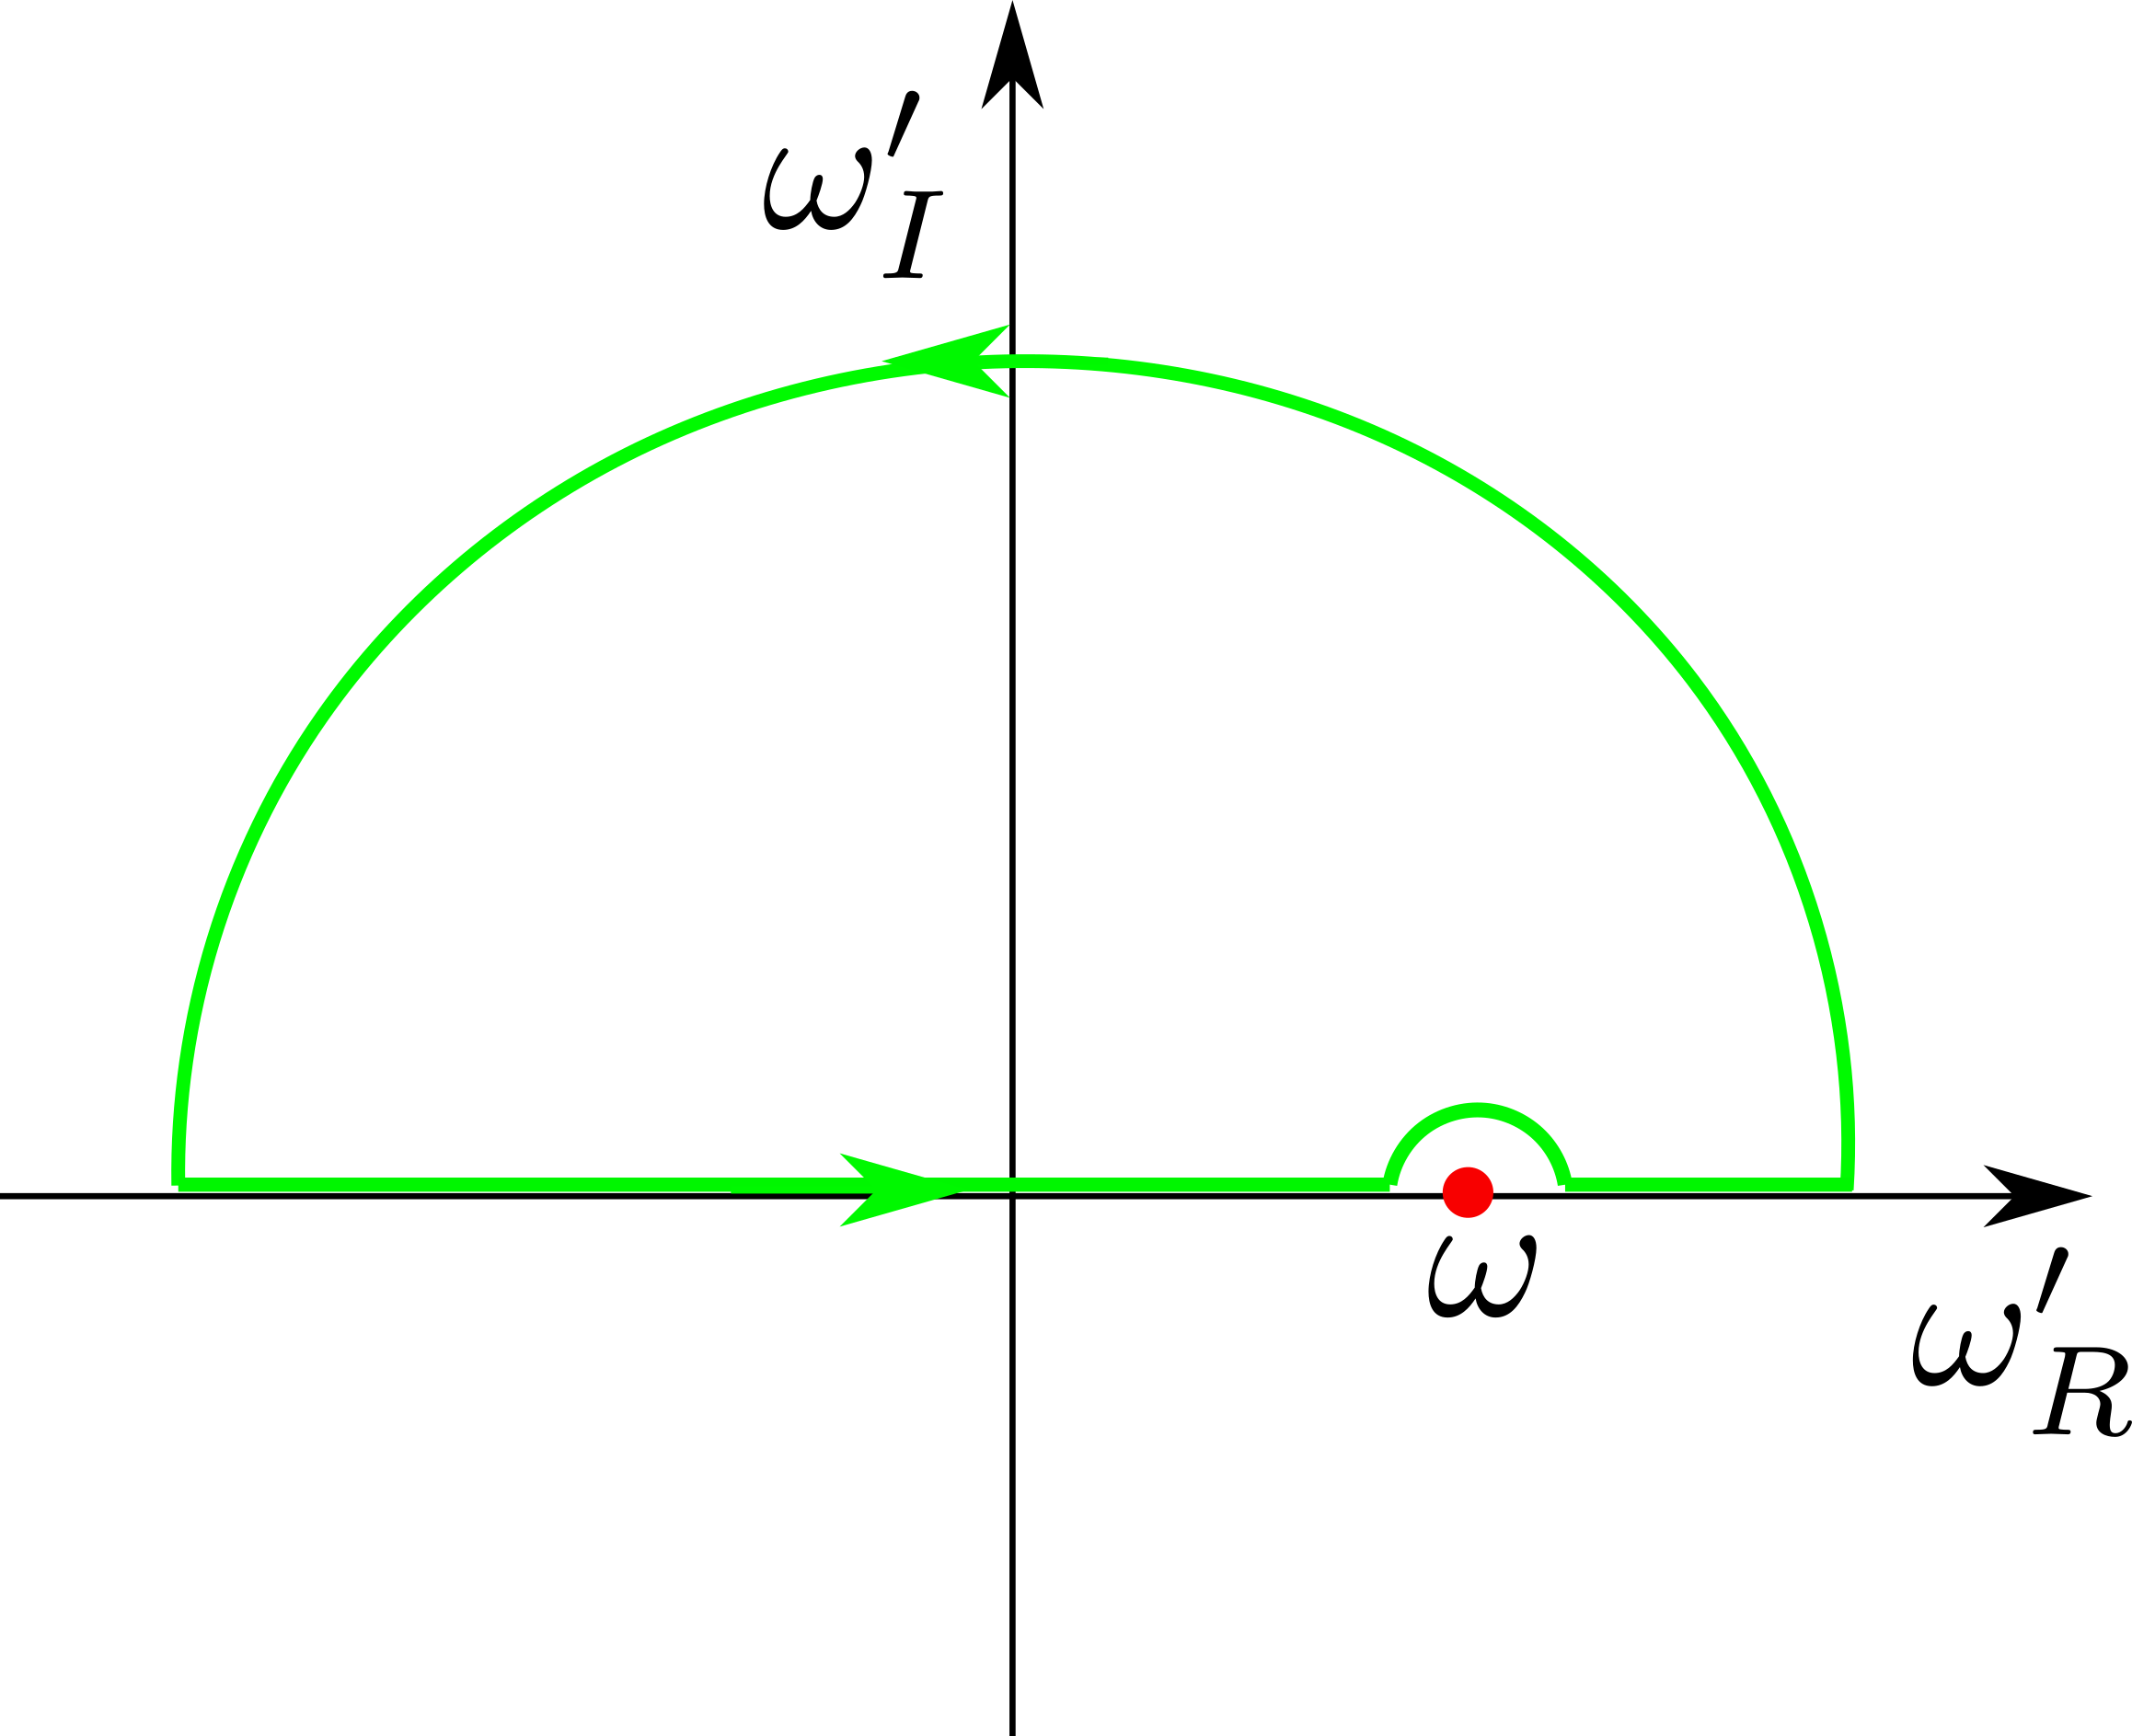
\includegraphics[width=2in]
{kramers-kronig/closed-path.png}
\caption{Closed integration contour $\gamma$ in $\omega'$ complex
plane. Used to prove Kramers-Kronig relations.}
\label{fig-closed-path-kkr}
\end{figure}

If $\gamma$ is the closed integration contour presented in Fig.\ref{fig-closed-path-kkr},
with the large semicircle having a radius $R\rarrow \infty$,
and the small semicircle having  a radius $\rho\rarrow 0$,
we must have

\beq
\int_{\gamma}d\omega'
 \frac{\chi(\omega')}{\omega'-\omega} =0
\eeq
The integral over the large semicircle 
tends to zero as $R\rarrow \infty$. 
As for the integral over the small 
semicircle 
$SC$, we 
can evaluate it as follows. Let

\beq
\omega'-\omega = \rho e^{i\theta}
\eeq
Then

\beqa
\int_{SC}d\omega'\frac{\chi(\omega')}{\omega'-\omega}
&=&
\chi(\omega)\int_{SC}\frac{d(\rho e^{i\theta})}{\rho e^{i\theta}}
\\
&=&
\chi(\omega)\int_{\pi}^{0}id\theta 
\\
&=&
\chi(\omega)(-i\pi)
\eeqa
Combining our results
for the integrals
over the various pieces of $\gamma$, 
we get
 
\beq
0=\int_{\gamma}d\omega'
 \frac{\chi(\omega')}{\omega'-\omega} =
 PP
 \int_{-\infty}^{\infty}d\omega'
  \frac{\chi(\omega')}{\omega'-\omega}
 -i\pi \chi(\omega)
\eeq

\qed

\begin{claim}(Kramers-Kronig relations assuming $\chi(t)$ is real)

If $\chi(t)$ is real, then the
KKR can be recast so that they only
contain integrals over positive, not negative, frequencies.

\beq
\chi_R =\frac{2}{\pi}
\int_0^\infty d\omega'\;\frac{\omega' \chi_I(\omega')}
{\omega^{'2}-\omega^2}
\eeq

\beq
\chi_I =-\frac{2}{\pi}
\int_0^\infty d\omega'\;\frac{\omega \chi_R(\omega')}
{\omega^{'2}-\omega^2}
\eeq
\end{claim}
\proof

Multiply by $(\omega'+\omega)$
the numerator and denominator
of the integrand of Eq.(\ref{eq-R-equals-int-I})
to get

\beqa
\chi_R(\omega) 
&=& \frac{1}{\pi}{\rm PP}
\int_{-\infty}^{\infty}d\omega'\; 
\frac{\chi_I(\omega')}{\omega'-\omega}
\\
&=&
 \frac{1}{\pi}{\rm PP}
\int_{-\infty}^{\infty}d\omega'\; 
\frac{(\omega'+\omega)\overbrace{\chi_I(\omega')}^{\text{odd function}}}{\omega^{'2}-\omega^2}
\\
&=&
 \frac{2}{\pi}{\rm PP}
\int_{0}^{\infty}d\omega'\; 
\frac{\omega'\chi_I(\omega')}{\omega^{'2}-\omega^2}
\eeqa

Multiply by $(\omega'+\omega)$
the numerator and denominator
of the integrand of Eq.(\ref{eq-I-equals-int-R})
to get

\beqa
\chi_I(\omega) 
&=& -\frac{1}{\pi}{\rm PP}
\int_{-\infty}^{\infty}d\omega'\; 
\frac{\chi_R(\omega')}{\omega'-\omega}
\\
&=&
 -\frac{1}{\pi}{\rm PP}
\int_{-\infty}^{\infty}d\omega'\; 
\frac{(\omega'+\omega)\overbrace{\chi_R(\omega')}^{\text{even function}}}{\omega^{'2}-\omega^2}
\\
&=&
- \frac{2}{\pi}{\rm PP}
\int_{0}^{\infty}d\omega'\; 
\frac{\omega\chi_R(\omega')}{\omega^{'2}-\omega^2}
\eeqa
\qed

\section{Damped Harmonic Oscillator Example}

From Chapters \ref{ch-greens-fun}
and \ref{ch-dynamical-sys}, a damped harmonic oscillator satisfies

\beq
\call x = f(t) 
\eeq
where

\beq
\call= \partial_t^2  + 2\gamma \partial_t + \omega^2_0
\eeq
and


\beq
f(t) = \frac{F_0}{m}\cos(\omega t +\delta)
\eeq
We also know that

\beq
x(t) = \int dt \chi(t -s)f(s)\;,\quad x(\omega)=
\chi(\omega) f(\omega)
\eeq

The Green's function $\chi(t-s)$
satisfies

\beq
\call\chi(t-s)=\delta(t-s)
\eeq
Using

\beq
\chi(t) =\int_{-\infty}^{\infty}\frac{d\omega}{2\pi}
e^{-i\omega t}\chi(\omega)
\;,\quad
\delta(t) =
\int_{-\infty}^{\infty}\frac{d\omega}{2\pi}
e^{-i\omega t}
\eeq
we get

\beq
\chi(\omega)(-\omega^{2} -i2\gamma\omega  +\omega_0^2)= 1
\eeq
so

\beq
\chi(\omega)=
\frac{1}{\omega_0^2-\omega^2 - i 2\gamma \omega}
\eeq
Hence,

\beq
\chi_R(\omega)=
\frac{\omega_0^2-\omega^2}{
(\omega_0^2-\omega^2)^2 - (2\gamma \omega)^2
}
\quad \text{(even function of $\omega$)}
\eeq
and

\beq
\chi_I(\omega)=
\frac{2\gamma \omega}{
(\omega_0^2-\omega^2)^2 - (2\gamma \omega)^2
}
\quad \text{(odd function of $\omega$, vanishes if $\gamma=0$)}
\eeq

Recall from Physics
that if $dW$ is an infinitesimal
amount of work,
$F$ is a force and $dx$ is
an infinitesimal displacement, 
\beq
dW = -Fdx
\eeq
Therefore, the {\bf power dissipation} is

\beq
P_{diss} = \frac{dW}{dt}  = F \dot{x}
\eeq
and its average over a time
interval $T$
that covers on full cycle is

\beq
\av{P_{diss}}=
\frac{1}{T}\int_0^T dt\; F(t) \dot{x}(t)
\eeq

\begin{claim}
For a damped harmonic oscillator driven by the force $F(t)=F_0\cos(\nu t)$,
the time averaged power dissipation is 

\beq
\av{P_{diss}}=
\frac{F_0^2 \nu\chi_I(\nu)}{2m} 
\eeq
\end{claim}
\proof
\beq
F(t) = F_0\cos(\nu t)=
 F_0 \left(
\frac{e^{i\nu t} + e^{-i\nu t}}{2}\right)\;,\;\;
f(t) = F(t)/m
\eeq

\beq
f(\omega)= 
\frac{F_0}{m}2\pi \left(
\frac{\delta(\omega-\nu) 
+ \delta(\omega +\nu)}{2}\right)
\eeq

\beq
x(\omega)=\chi(\omega)\frac{F_0}{m}
2\pi\left(\frac{\delta(\omega-\nu) + \delta(\omega + \nu)}{2}
\right)
\eeq

\beqa
x(t)&=&\int_{-\infty}^{\infty}
\frac{d\omega}{2\pi}\; e^{-i\omega t}x(\omega)
\\
&=&
\frac{F_0}{2m}\left(\chi(\nu)  e^{-i\nu t}
+ \underbrace{\chi(-\nu)}_{\chi^*(\nu)}  e^{i\nu t}\right)
\\
&=&
 \chi(\nu) \frac{F_0}{2m} e^{-i\nu t} + c.c.
\eeqa

\beq
\dot{x}(t)=
(-i\nu)\chi(\nu) \frac{F_0}{2m} e^{-i\nu t}
+ c.c.
\eeq

\beqa
\av{P_{diss}}&=&
\frac{1}{T}\int_0^T dt\; 
\left(\frac{F_0}{2}e^{i\nu t} + c.c.
\right)
\left(
-i\nu\chi(\nu) \frac{F_0}{2m} e^{-i\nu t}
+ c.c.\right)
\\
&=&
\left(\frac{F_0^2}{4m}
\right) \nu\left[-i\chi(\nu)+c.c.
\right]\quad\text{(other terms average out to 0)}
\\
&=&
\left(\frac{F_0^2}{2m}
\right) \nu \chi_I(\nu)
\eeqa
\qed